% =====================================================================
%  Journal paper (IOP template) — expanded from the NILES 2026 submission
%  Core = NilesConf/submission/main.tex (audited prose) + 3 new sections.
%  Prose humanized by the team (rewrite/ pack), fix-integrated and merged
%  2026-07-13; numbers and citations re-verified against thesis ch. 5 /
%  phase-2 reports. Do NOT edit numbers without re-auditing.
%  For double-anonymous review: \documentclass[anonymous]{iopjournal}
%  and genericize the E-JUST sentence in the conclusion.
% =====================================================================
\documentclass{iopjournal}

\usepackage{amsmath,amssymb}
\usepackage{booktabs}
\usepackage{tikz}
\usetikzlibrary{positioning, arrows.meta, calc}
% all figure files sit next to main.tex (IOP submission system: no subfolders)

\begin{document}

\articletype{Paper}

\title{Fundamental limits of compressing CSI-based indoor localization for edge deployment: capacity, robustness, and cross-session generalization}

% TODO before submission: append \orcid{....-....-....-....} after "Ehab Elshazly$^{1,*}$"
% once Prof. Ehab provides his ORCID iD (co-authors have none yet — that is fine).
\author{Ehab Elshazly$^{1,*}$, Abdulrahman Mahmoud Ali Ebrahim$^{1}$, Ahmed Emadeldin Abdelsallam Haggag$^{1}$ and Fadwa Yasser Khalil Mahmoud$^{1}$}

\affil{$^1$Department of Computer Science and Engineering, Egypt-Japan University of Science and Technology (E-JUST), Alexandria, Egypt}

\affil{$^*$Author to whom any correspondence should be addressed.}

\email{ehab.elshazly@ejust.edu.eg}

\keywords{indoor localization, WiFi sensing, channel state information, knowledge distillation, model compression, edge computing, robustness}

\begin{abstract}
Positioning indoors is important for the management of hospital equipment, patients, and navigating robots within a facility. However, GPS-based systems do not perform well indoors. The current state of the art in indoor localization uses deep learning to transform WiFi Channel State Information (CSI) measurements from four access points into a heatmap of the device location with sub-meter accuracy. This model, known as DLoc, contains 16.5 million parameters, however, which makes it unsuitable for most edge devices. In this paper, we ask: what are the fundamental limits of compressing CSI-based indoor localization for edge deployment? Using the public WILD dataset, we study five models spanning three orders of magnitude in parameter count, from a 47K-parameter convolutional network to the 16.5M-parameter DLoc model itself. Each student model is trained both independently and with knowledge distillation from DLoc as a ``teacher'' model. Our results reveal a capacity floor near 2 million parameters, below which localization accuracy collapses and knowledge distillation cannot recover it. Additionally, the model architecture must preserve the two-dimensional nature of the CSI measurements. Above the capacity floor, reducing the model size does not impact localization accuracy: the distilled MobileNetV2-UNet reaches a median error of 0.640 meters, tying the published accuracy of DLoc with 6.8 times fewer parameters and 56 times less computation. Results show that skip connections provide robustness to noise in the signal, that knowledge distillation provides robustness under distribution shift and access-point failure, and that below the capacity floor distillation actively harms robustness. Additionally, the distilled MobileNetV2-UNet outperforms the other student models on test sessions never seen during training, and its standalone variant remains within 0.14 meters of DLoc under a strict leave-one-session-out protocol. Thus, our results demonstrate that accurate and robust indoor localization does not require a large model or a great deal of computational power.
\end{abstract}

\section{Introduction}
\label{sec:intro}
While GPS offers accurate positioning of objects when they are outdoors, its accuracy disappears when the objects are indoors. Hence, indoor localization has been an active area of research for the last two decades, supporting applications that range from tracking factory assets~\cite{digitaltwin2025framework} to guiding robots and monitoring patients.

The predominant technique for indoor localization uses WiFi signal data and analyzes the Channel State Information (CSI) from access points~\cite{ayyalasomayajula2020deep} to determine the time-of-flight (ToF) and angle-of-arrival (AoA) of the signals with sub-meter accuracy. The deep learning-based DLoc model~\cite{ayyalasomayajula2020deep} transforms the CSI data to produce a heatmap that depicts the location of the device within the floor plan of the building.

The current model has a major drawback of requiring a large amount of training data and a deep learning model with 16.5M parameters to function, making it difficult to deploy within standard WiFi gateways, access points, or smartphones. For CSI-based indoor localization to be employed within the existing WiFi networking hardware in every building, such a model would have to be compressed by an order of magnitude. This paper is therefore organized around the question: \emph{what are the fundamental limits of compressing CSI-based indoor localization for edge deployment?} We break this question into six concrete sub-questions:
\begin{enumerate}
  \item How small can the model become before accuracy collapses?
  \item Does knowledge distillation recover lost accuracy?
  \item Which architectures preserve spatial localization?
  \item Which models remain robust under signal degradation?
  \item Which models generalize across environmental changes?
  \item What is the accuracy--efficiency trade-off?
\end{enumerate}

To answer them, we evaluate a ladder of ``student'' models of increasing capacity ranging from 47K to over 2M parameters---including models of the TinyCNN, Mamba, MobileNetV2 and MobileNetV2-UNet architectures---against the 16.5M-parameter DLoc model on the WILD dataset using both standalone and knowledge-distillation training protocols. Specifically, our work makes three contributions to the field: firstly, through a capacity analysis in section~\ref{sec:capacity}, which allows us to determine the minimum model capacity necessary to solve the CSI-to-heatmap problem; secondly, through a robustness analysis in section~\ref{sec:robustness}, which investigates the impact of corruption on the input CSI signals; and finally, through a cross-session generalization analysis in section~\ref{sec:crosssession}, which assesses the impact of environmental changes on the models' ability to localize. Together with the statistical stability and efficiency analysis in section~\ref{sec:efficiency}, these contributions indicate that it is possible to achieve accuracy comparable to the DLoc model at a fraction of its computational cost.

\section{Related work}
\label{sec:related}
Indoor localization using WiFi Channel State Information (CSI) has long been studied~\cite{ayyalasomayajula2020deep} and remains an area of active research. Some approaches to WiFi localization include the use of transformers to account for non-line-of-sight environments~\cite{masrur2025transforming}, as well as techniques like meta-learning~\cite{owfi2023meta} and few-shot learning~\cite{tiku2023fewshot} to account for long-term changes in the signal environment. Related efforts have explored approaches to domain adaptation~\cite{jiao2025robust}, angle-of-arrival calibration~\cite{adaptiveaoa2026learning}, interpretability~\cite{gufran2025towards}, and data augmentation~\cite{serbetci2024wireless}. While these approaches primarily focus upon maximizing the accuracy or generalizability of localization approaches, we focus upon a different and equally important aspect of localization systems: model efficiency.

Model efficiency is often improved through the application of knowledge distillation, wherein a smaller model is trained to mimic the behavior of a much larger model~\cite{hinton2015distilling}. Knowledge distillation has long been employed in the context of image classification with deep neural networks, but has also been applied to other computer vision tasks such as object detection~\cite{zheng2023localization} and cross-modal localization~\cite{nazaraliyev2025mambaloc}. Our approach to knowledge distillation is different from these previous methods, however, in that our student model learns to mimic the teacher model's heatmaps as targets to minimize rather than the classification logits.

The student architectures employ a range of well-established techniques from image recognition fields, such as residual connections~\cite{he2016resnet}, inverted residuals as employed by MobileNetV2~\cite{sandler2018mobilenetv2}, skip connections as in U-Net~\cite{ronneberger2015unet}, and state-space models such as Mamba~\cite{gu2023mamba,visualmamba2024survey}. Furthermore, given the importance of lightweight models in the contexts of green WiFi sensing~\cite{greenwireless2026survey} and TinyML deployment~\cite{tinyml2022iot}, such models are of direct practical interest.

Yet high accuracy on a relatively clean and curated dataset does not by itself indicate that the models are to be relied upon in real environments with potentially corrupted CSI measurements~\cite{hendrycks2019robustness}. Therefore, in addition to the models trained on the clean dataset, we also evaluate the models' robustness against various forms of corruption to the measurements that were not seen during training.

\section{Method}
\label{sec:method}
\subsection{The DLoc system and the WILD dataset}
The DLoc system~\cite{ayyalasomayajula2020deep} takes four AoA--ToF images from four APs and outputs a single-channel heatmap whose peak is the predicted location of the device. Its deep learning model uses a ResNet encoder with two decoders---a location decoder and a consistency (offset) decoder---for a total of 16.5\,M parameters.

The WILD dataset, collected in Jacobs Hall at UCSD~\cite{ayyalasomayajula2020deep}, includes five sessions of data collection that are summarized in table~\ref{tab:sessions}. Two sessions performed in July contributed to 17{,}574 training samples and 4{,}260 test samples that were collected in-distribution from the training area. The other three sessions took place in August, three weeks after the July sessions, and with various alterations to the environment in which the dataset was collected. Environmentally-altered sessions included newly-arranged furniture (11{,}201 samples), new furniture of a different kind (8{,}754 samples), and the addition of an aluminum reflector to the environment (5{,}486 samples). The leave-one-session-out cross-validation splits the dataset into three folds, where each fold trains on the samples from the two July sessions and two August sessions, and tests on the samples from the August session that was not used for training within that fold, following the same protocol as the published DLoc evaluation.

\begin{table}
\caption{The five WILD collection sessions. Sessions 1+2 together provide 17{,}574 training samples; the Session-2 figure shown is its held-out test split.}
\label{tab:sessions}
\centering
\begin{tabular}{l l r l}
\hline
\textbf{Session} & \textbf{Tag} & \textbf{Samples} & \textbf{Condition} \\
\hline
1 & \texttt{jacobs\_Jul28}         & ---      & training (reference conditions) \\
2 & \texttt{jacobs\_Jul28\_2}      & 4{,}260  & in-distribution test (1\,h later, identical) \\
3 & \texttt{jacobs\_Aug16\_1}      & 11{,}201 & furniture rearrangement \\
4 & \texttt{jacobs\_Aug16\_3}      & 8{,}754  & different furniture configuration \\
5 & \texttt{jacobs\_Aug16\_4\_ref} & 5{,}486  & aluminum reflector (specular multipath) \\
\hline
\end{tabular}
\end{table}

\subsection{Student network architectures}
\label{sec:students}
Since each student network has the same inputs and outputs as the teacher model, any of the student models can be used to substitute for the DLoc system. Each model is summarized in table~\ref{tab:models}.

MobileNetV2 (2.27\,M parameters) uses the MobileNetV2 backbone~\cite{sandler2018mobilenetv2}, originally designed for image representation and classification, which is adapted to accept the four-channel CSI input from the APs. The MobileNetV2-UNet (2.41\,M) model is similar to the MobileNetV2 model, but includes skip connections in the style of the U-Net architecture~\cite{ronneberger2015unet} that allow for the direct concatenation of feature maps of encoder layers to those of the decoder layers having the same spatial resolution (figure~\ref{fig:unet}). This U-Net model allows for more information regarding spatial features of the input CSI measurements to be fed into the decoder model. The TinyCNN model has 47\,K parameters and includes three convolutional and two fully connected layers ($351\times$ compression of the number of parameters relative to DLoc); it is included to probe the lower limit of viable model size. Finally, the Mamba model has 0.65\,M parameters, and applies a different deep learning model altogether: a selective state-space model~\cite{gu2023mamba} that treats the CSI measurements from the APs as one-dimensional sequences rather than images, included to test whether this different inductive bias is competitive for the CSI-to-heatmap problem.

\begin{table}
\caption{The capacity ladder: the DLoc teacher and the four student architectures, with computational cost at batch size 1. The DLoc figures are for its test-time path (encoder + location decoder). Mamba FLOPs/latency are omitted as it is non-competitive (section~\ref{sec:capacity}).}
\label{tab:models}
\centering
\begin{tabular}{l r c l r r r}
\hline
\textbf{Model} & \textbf{Params} & \textbf{Compr.} & \textbf{Architecture} & \textbf{FLOPs} & \textbf{CPU (ms)} & \textbf{GPU (ms)} \\
\hline
DLoc (teacher)   & 16.5M & $1\times$   & ResNet enc.\ + 2 decoders & 81.06G & 270.9 & 16.2 \\
MobileNetV2      & 2.27M & $7.2\times$ & inverted residuals        & 1.28G  & 17.9  & 6.3 \\
MobileNetV2-UNet & 2.41M & $6.8\times$ & + U-Net skip connections  & 1.45G  & 27.2  & 4.5 \\
Mamba            & 0.65M & $25\times$  & 1D selective state-space  & ---    & ---   & --- \\
TinyCNN          & 47K   & $351\times$ & 3 conv + 2 FC layers      & 0.66G  & 9.1   & 1.5 \\
\hline
\end{tabular}
\end{table}

\begin{figure}
\centering
\resizebox{0.8\textwidth}{!}{% ============================================================================
%  MobileNetV2-UNet architecture — \input-able body (no \documentclass).
%  Requires in the master preamble: \usepackage{tikz} and
%  \usetikzlibrary{positioning, arrows.meta, calc}.  Colours are defined here
%  so the figure is self-contained.  Layer specs from code/models/student_unet.py.
% ============================================================================
\definecolor{cEnc}{RGB}{142,202,230}
\definecolor{cBottle}{RGB}{33,102,172}
\definecolor{cDec}{RGB}{69,123,157}
\definecolor{cHead}{RGB}{188,108,37}
\definecolor{cSkip}{RGB}{42,157,143}
\definecolor{cIO}{RGB}{230,57,70}

\begin{tikzpicture}[
  font=\small,
  >={Stealth[length=2.4mm]},
  block/.style={rectangle, rounded corners=2pt, draw=black!70, thick,
                minimum height=11mm, minimum width=13mm, align=center,
                text=white, font=\normalsize\bfseries},
  enc/.style={block, fill=cEnc, text=black},
  bottle/.style={block, fill=cBottle},
  dec/.style={block, fill=cDec},
  head/.style={block, fill=cHead},
  io/.style={rectangle, rounded corners=1pt, draw=black!70, thick,
             minimum height=13mm, minimum width=12mm, align=center,
             fill=cIO!12, font=\normalsize},
  flow/.style={->, black!75, thick},
  skipline/.style={->, cSkip, very thick, dashed},
]
\node[io] (in) {Input\\$4{\times}161{\times}361$};
\node[enc,    right=5mm of in]  (inc) {inc\\$4{\to}32$\\/2};
\node[enc,    right=4mm of inc] (e1)  {enc1\\$24$};
\node[enc,    right=4mm of e1]  (e2)  {enc2\\$32$};
\node[enc,    right=4mm of e2]  (e3)  {enc3\\$96$};
\node[bottle, right=4mm of e3]  (e4)  {enc4\\$320$};
\node[dec,  right=8mm of e4] (d1) {dec1\\$416{\to}128$};
\node[dec,  right=4mm of d1]  (d2) {dec2\\$160{\to}64$};
\node[dec,  right=4mm of d2]  (d3) {dec3\\$88{\to}32$};
\node[head, right=4mm of d3]  (hd) {head\\$32{\to}1$\\Sigmoid};
\node[io,   right=5mm of hd]  (out) {Output\\$1{\times}161{\times}361$};
\draw[flow] (in)--(inc); \draw[flow] (inc)--(e1); \draw[flow] (e1)--(e2);
\draw[flow] (e2)--(e3);  \draw[flow] (e3)--(e4);  \draw[flow] (e4)--(d1);
\draw[flow] (d1)--(d2);  \draw[flow] (d2)--(d3);  \draw[flow] (d3)--(hd);
\draw[flow] (hd)--(out);
\draw[skipline] (e3.north) to[out=90,in=90]
      node[above,font=\small,text=cSkip]{skip 96} (d1.north);
\draw[skipline] (e2.north) to[out=90,in=90]
      node[above,font=\small,text=cSkip]{skip 32} (d2.north);
\draw[skipline] (e1.north) to[out=90,in=90]
      node[above,font=\small,text=cSkip]{skip 24} (d3.north);
\node[text=black!60, font=\small, below=2.5mm of e2.south] {MobileNetV2 encoder (pretrained, 4-ch input)};
\node[text=black!60, font=\small, below=2.5mm of d2.south] {U-Net decoder (upsample $+$ skip concat)};
\end{tikzpicture}
}
\caption{The MobileNetV2-UNet student. A MobileNetV2 encoder (light blue) downsamples the four-channel input; a decoder (dark blue) upsamples back to full resolution; teal dashed arcs are U-Net skip connections bypassing the bottleneck.}
\label{fig:unet}
\end{figure}

\subsection{Knowledge-distillation framework}
For each input, the fixed DLoc teacher network generates a soft target heatmap $y_T$. Each student model trains independently (using the ground-truth label $y$ alone) and within distilled mode, minimizing
\begin{equation}
\mathcal{L} = \alpha\,\mathrm{MSE}(\hat{y}, y) + \beta\,\mathrm{MSE}(\hat{y}, y_T),
\label{eq:loss}
\end{equation}
for coefficients $\alpha$ and $\beta$ set to 0.7 and 0.3, respectively. The teacher network's outputs are pre-computed offline and used as fixed targets during the training of each student model; the teacher itself never runs during training. Because the teacher network's targets are heatmaps rather than one-hot maps, its output is ``soft''---it distributes its probability mass around the true object location. This soft output helps regularize each student model during training.

\subsection{Evaluation metrics}
The localization error $e$ is the Euclidean distance between the two heatmap peaks,
\begin{equation}
e = 0.1 \cdot \lVert \arg\max(\hat{y}) - \arg\max(y) \rVert_2 \;\; [\mathrm{m}],
\label{eq:err}
\end{equation}
scaled by a factor of 0.1 to convert pixels to meters. Following previous work in the field~\cite{ayyalasomayajula2020deep}, the median of $e$ along with the 90th and 99th percentile values of $e$ are reported. Because the localization error is discrete and quantized in steps of $0.1\sqrt{n}$ meters, two models may have the same median error but different distributions of error. Therefore, presenting the error in percentiles provides a more complete description of the error each model makes in localizing the object of interest.

\section{Implementation}
\label{sec:implementation}
All models are implemented in PyTorch. TinyCNN and MobileNetV2 are trained with the Adam optimizer with a learning rate of $10^{-4}$ and a batch size of 64 for 50 epochs, while MobileNetV2-UNet is trained for 120 epochs with cosine annealing and step decay schedulers. Finally, DLoc uses the Adam optimizer with $\beta_1{=}0.5$ and a StepLR scheduler with $\gamma{=}0.9$. The models with the lowest test error are chosen from each architecture. While the training occurs on rented NVIDIA H100 GPUs, the latency measurements in table~\ref{tab:models} are collected on a desktop GPU with an RTX~3060 card. Furthermore, since the teacher model is not retrained within the leave-one-session-out (LOSO) procedure, the MobileNetV2-UNet runs in standalone mode during this procedure to maintain comparability with the reported DLoc results. All the code, weights, training logs and teacher model outputs are archived in a public repository to allow anyone to reproduce the results.

\section{Capacity analysis: how much model capacity is actually required for CSI-based indoor localization?}
\label{sec:capacity}
Rather than considering each of the five models in table~\ref{tab:models} in isolation, collectively they represent a single study of model capacity. Together they span the parameter count range from 47\,K to 16.5\,M (from $351\times$ to $1\times$ model compression), and each was trained and tested on the same test split (Session 2).

Table~\ref{tab:indist} reports on the in-distribution localization errors of each of these models, figure~\ref{fig:cdf} plots the CDF of their errors, and figure~\ref{fig:pareto} plots each model on the accuracy--size plane.

\begin{table}
\caption{In-distribution accuracy across the capacity ladder (Session-2 test set, $N{=}4{,}260$; best in \textbf{bold}; published DLoc from~\cite{ayyalasomayajula2020deep}). Student models trained for 50 epochs; MobileNetV2-UNet variants for 120 epochs.}
\label{tab:indist}
\centering
\begin{tabular}{l r l c c c}
\hline
\textbf{Model} & \textbf{Params} & \textbf{Mode} & \textbf{Median (m)} & \textbf{P90 (m)} & \textbf{P99 (m)} \\
\hline
DLoc (published) & 16.5M & ---        & \textbf{0.64} & 1.6 & 3.2 \\
DLoc (our repro) & 16.5M & ---        & 0.707 & ${\sim}1.6$ & ${\sim}4.0$ \\
\hline
MobileNetV2      & 2.27M & Standalone & 0.707 & 1.616 & 3.992 \\
MobileNetV2      & 2.27M & Distilled  & 0.707 & 1.612 & 4.003 \\
\hline
MobileNetV2-UNet & 2.41M & Standalone (Cosine) & \textbf{0.640} & 1.523 & 2.750 \\
MobileNetV2-UNet & 2.41M & Standalone (Step)   & \textbf{0.640} & 1.552 & 2.918 \\
MobileNetV2-UNet & 2.41M & Distilled (Cosine)  & \textbf{0.640} & \textbf{1.513} & \textbf{2.587} \\
\hline
Mamba            & 0.65M & Standalone & 10.56 & 20.0 & 28.3 \\
\hline
TinyCNN          & 47K   & Standalone & 3.922 & 13.919 & 23.244 \\
TinyCNN          & 47K   & Distilled  & 3.706 & 14.784 & 25.101 \\
\hline
\end{tabular}
\end{table}

\begin{figure}
\centering
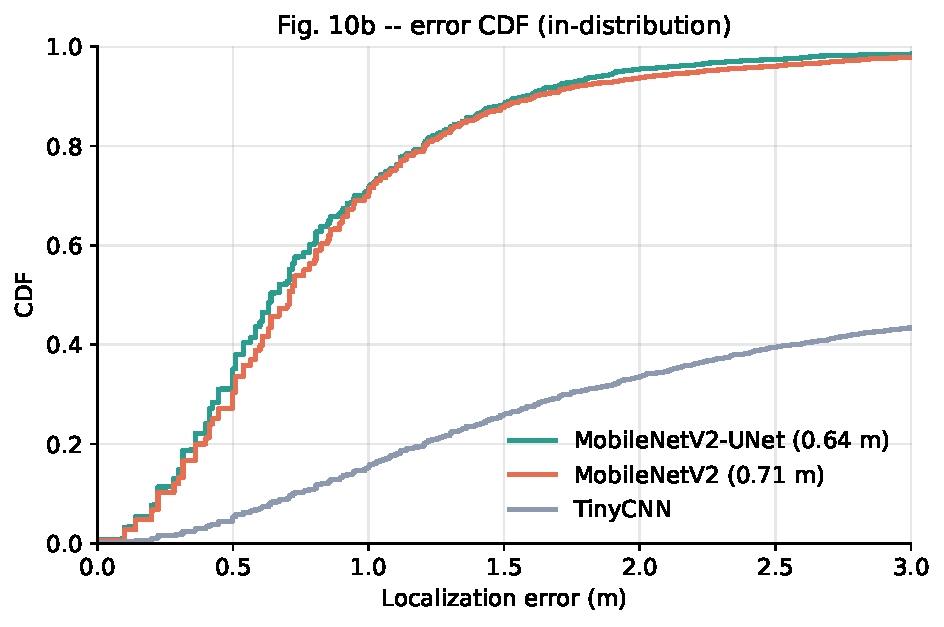
\includegraphics[width=0.62\textwidth]{cdf_fig10b.pdf}
\caption{Cumulative distribution of in-distribution localization error. The MobileNetV2-UNet (0.640\,m median) lies above the plain MobileNetV2 (0.707\,m) across the full range, while TinyCNN trails far behind, never reaching the 0.8 CDF level within 3\,m.}
\label{fig:cdf}
\end{figure}

\begin{figure}
\centering
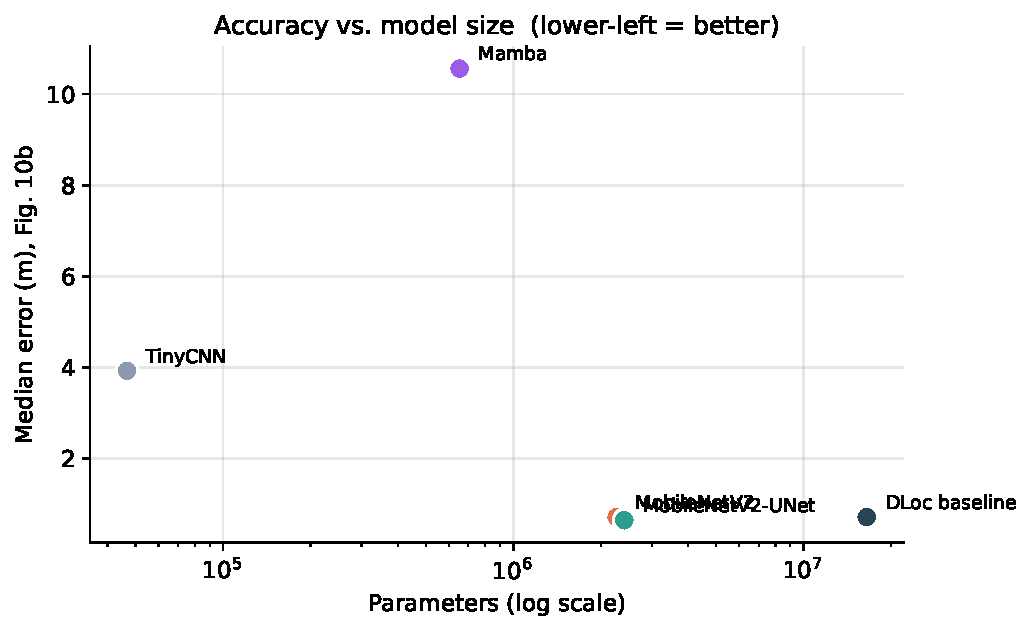
\includegraphics[width=0.6\textwidth]{compression_pareto.pdf}
\caption{Accuracy versus model size. The MobileNetV2-UNet sits at the favorable lower-left of the accuracy--size plane, achieving the best median error among all models at a fraction of the DLoc parameter count; Mamba sits at the top of the plane despite a mid-range parameter count, showing that architecture, not size alone, determines feasibility.}
\label{fig:pareto}
\end{figure}

\subsection{DLoc is over-parameterized in-distribution}
The MobileNetV2 model achieves the same result (median error of 0.707\,m) as our DLoc reproduction but uses $7.2\times$ fewer parameters. Furthermore, the MobileNetV2-UNet model achieves the lowest median error of 0.640\,m (9.5\% below MobileNetV2 and our DLoc reproduction, and level with DLoc's published 0.64\,m~\cite{ayyalasomayajula2020deep}) with only 2.41\,M parameters. Thus, the introduction of skip connections allows a student model to outperform its teacher model using $6.8\times$ fewer parameters. Figure~\ref{fig:heatmaps_indist} illustrates representative results from the MobileNetV2-UNet. The learning rate schedule had a small effect on the performance of this model (switching from step decay to cosine annealing for MobileNetV2-UNet led to a slight reduction in the tail percentiles of prediction errors; the 99th percentile error went from 2.918\,m to 2.750\,m); the architecture has the dominant effect on localization error.

\begin{figure}
\centering
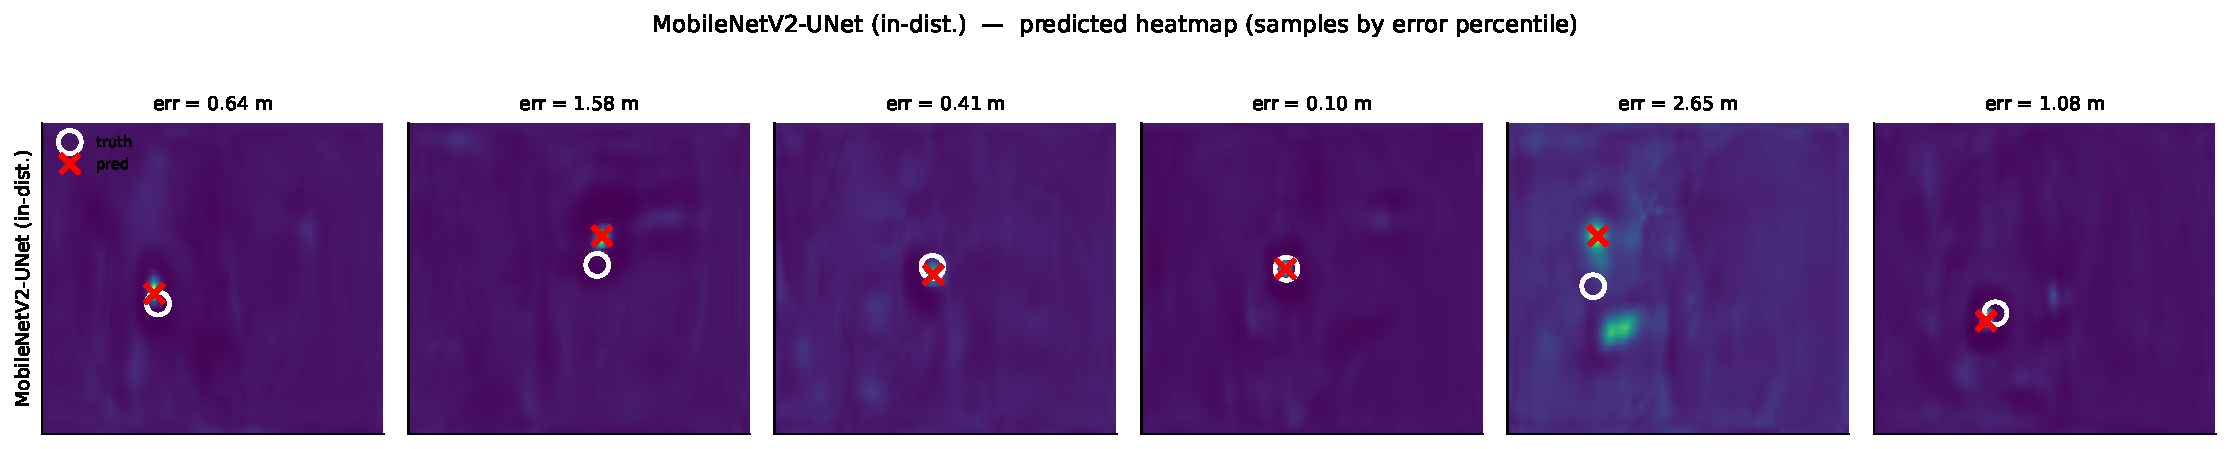
\includegraphics[width=\textwidth]{heatmaps_unet_fig10b.pdf}
\caption{Qualitative in-distribution predictions of the MobileNetV2-UNet. Each panel shows the predicted heatmap for a test sample drawn at a given error percentile; the white circle marks the ground-truth peak and the red cross the predicted peak. Low-error cases (left) show tight, single-mode predictions; the high-error case shows a multimodal heatmap where the chosen peak is displaced.}
\label{fig:heatmaps_indist}
\end{figure}

\subsection{Accuracy collapses below a capacity floor of roughly 2M parameters}
The TinyCNN model with 47\,K parameters reaches a median error of 3.922\,m---more than 5 times the baseline error. Its three convolutional layers appear to be insufficient for learning both the features within each AP and the spatial structure of the location. Thus, the capacity floor for this problem appears to be around 2 million parameters; any model smaller than this parameter count will not achieve accurate localization results, no matter how much training is performed on it.

Crucially, knowledge distillation does not rescue an under-capacity model. The distilled TinyCNN has a median error that is only marginally lower than the standalone model (from 3.922\,m to 3.706\,m), and its percentiles in the tail of the distribution of errors have worsened (from 23.244\,m to 25.101\,m). Thus, knowledge distillation does not help a model that lacks the capacity to hold the knowledge of the teacher. Knowledge distillation cannot help the under-capacity model in this way, nor does it improve the in-distribution accuracy of models above the floor (both MobileNetV2 and MobileNetV2-UNet have identical standalone and distilled median errors in table~\ref{tab:indist}). Within the training set, the teacher's predictions are nearly identical to the ground truth; there is no value in distilling knowledge within this range of training examples. The value of knowledge distillation only emerges outside of the training distribution of examples (sections~\ref{sec:robustness} and~\ref{sec:crosssession}).

\subsection{Architecture must preserve two-dimensional spatial structure}
The reason that Mamba failed to learn the task of localizing objects within the environment is its architecture. Mamba has 14 times as many parameters as the TinyCNN, yet it is the worst-performing model in table~\ref{tab:indist} (median error of 10.56\,m). Mamba treats the CSI measurements as a one-dimensional sequence, whereas the target is a two-dimensional spatial heatmap; flattening the input destroys the spatial locality that the task depends on. The model attains its best accuracy at the very first epoch of training, and the errors on both the training and test sets continue to rise together in each following epoch; this rules out overfitting and indicates that Mamba is not well-suited to the problem of localizing objects within the environment. The other architectures that treat the input CSI as an image have preservation of spatial information in their architecture (especially the U-Net, which uses skip connections); these models have better performance in the tail of their distribution of predicted errors.

The capacity required to learn the localization task in the indoor environment is around 2M parameters of two-dimensional convolutional capacity---an order of magnitude less than DLoc uses for the same task, but not less than that floor, nor in an arbitrary neural network architecture.

\section{Robustness analysis: which compression strategy produces the most robust localization model?}
\label{sec:robustness}
Each of the localizer models that are deployed will encounter signal conditions that were never contained within the training set that was curated for each model~\cite{hendrycks2019robustness}. The CSI inputs are therefore corrupted at test time only, with various corruption schemes (per-AP and random AP dropout, Gaussian noise of $\sigma \in \{0.1, 0.2\}$, attenuation, and spatial blur), and each model is re-evaluated without retraining. The results of each model are presented in tables~\ref{tab:robust_mobilenet}--\ref{tab:robust_unet}, with table~\ref{tab:noise_summary} summarizing the results for models that were corrupted with Gaussian noise.

\begin{table}
\caption{Robustness evaluation --- MobileNetV2 (2.27M). \textbf{Bold} = distilled beats standalone.}
\label{tab:robust_mobilenet}
\centering
\begin{tabular}{l c c c c c c c c}
\hline
 & \multicolumn{4}{c}{\textbf{Standalone}} & \multicolumn{4}{c}{\textbf{Distilled}} \\
\textbf{Condition} & \textbf{Med.} & \textbf{P90} & \textbf{P99} & \textbf{Mean} & \textbf{Med.} & \textbf{P90} & \textbf{P99} & \textbf{Mean} \\
\hline
Normal                 & 0.707 & 1.616 & 3.992  & 0.900 & 0.707 & 1.612 & 4.003  & 0.896 \\
Noise $\sigma{=}0.1$   & 16.368& 20.939& 25.196 & 16.557& \textbf{4.769} & \textbf{12.310}& \textbf{21.122} & \textbf{5.953} \\
Noise $\sigma{=}0.2$   & 16.307& 20.748& 25.188 & 16.503& \textbf{5.369} & \textbf{20.508}& 26.014 & \textbf{7.896} \\
Random 2-AP dropout    & 2.402 & 11.691& 22.997 & 4.468 & 2.516 & \textbf{11.631}& \textbf{21.091} & \textbf{4.434} \\
Atten.\ $0.5\times$    & 1.342 & 4.211 & 14.831 & 2.181 & 1.500 & 6.185 & 22.612 & 2.828 \\
Blur $k{=}5$           & 0.849 & 2.121 & 12.033 & 1.281 & 0.854 & \textbf{1.924} & \textbf{5.839}  & \textbf{1.125} \\
\hline
\end{tabular}
\end{table}

\begin{table}
\caption{Robustness evaluation --- TinyCNN (47K). Distillation \emph{harms} dropout and attenuation robustness.}
\label{tab:robust_tinycnn}
\centering
\begin{tabular}{l c c c c c c c c}
\hline
 & \multicolumn{4}{c}{\textbf{Standalone}} & \multicolumn{4}{c}{\textbf{Distilled}} \\
\textbf{Condition} & \textbf{Med.} & \textbf{P90} & \textbf{P99} & \textbf{Mean} & \textbf{Med.} & \textbf{P90} & \textbf{P99} & \textbf{Mean} \\
\hline
Normal              & 3.922 & 13.919& 23.244 & 5.833 & 3.706 & 14.784& 25.101 & 6.048 \\
Random 1-AP dropout & 7.940 & 16.858& 23.405 & 8.580 & 13.648& 24.502& 28.228 & 12.922\\
Noise $\sigma{=}0.1$& 9.457 & 17.049& 25.018 & 9.946 & 9.439 & 16.568& 23.965 & 9.921 \\
Atten.\ $0.5\times$ & 9.708 & 17.593& 22.233 & 10.318& 18.532& 26.196& 28.343 & 17.829\\
\hline
\end{tabular}
\end{table}

\begin{table}
\caption{Robustness evaluation --- MobileNetV2-UNet (2.41M), cosine scheduler. \textbf{Bold} = best of the pair.}
\label{tab:robust_unet}
\centering
\begin{tabular}{l c c c c c c c c}
\hline
 & \multicolumn{4}{c}{\textbf{Standalone}} & \multicolumn{4}{c}{\textbf{Distilled}} \\
\textbf{Condition} & \textbf{Med.} & \textbf{P90} & \textbf{P99} & \textbf{Mean} & \textbf{Med.} & \textbf{P90} & \textbf{P99} & \textbf{Mean} \\
\hline
Normal              & 0.640 & 1.581 & 3.651  & 0.851 & 0.640 & \textbf{1.513} & \textbf{3.587}  & \textbf{0.829} \\
Noise $\sigma{=}0.1$& \textbf{3.000}& \textbf{8.310}& \textbf{13.873}& \textbf{3.878}& 3.469 & 10.473& 18.261 & 4.678 \\
Noise $\sigma{=}0.2$& 5.741 & \textbf{10.645}& \textbf{18.137} & \textbf{6.050} & \textbf{5.320} & 12.003& 17.948 & 6.135 \\
Random 2-AP dropout & 3.324 & 13.012& 22.080 & 5.228 & \textbf{2.730}& \textbf{8.203}& \textbf{13.396}& \textbf{3.711}\\
Blur $k{=}5$        & 0.671 & 1.603 & \textbf{3.716}  & 0.859 & \textbf{0.656}& \textbf{1.526}& 3.943 & \textbf{0.841} \\
\hline
\end{tabular}
\end{table}

\begin{table}
\caption{Gaussian-noise robustness summary ($\sigma = 0.1$). \textbf{Bold} = best.}
\label{tab:noise_summary}
\centering
\begin{tabular}{l l c c}
\hline
\textbf{Model} & \textbf{Mode} & \textbf{Median (m)} & \textbf{P90 (m)} \\
\hline
MobileNetV2      & Standalone & 16.368 & 20.939 \\
MobileNetV2      & Distilled  & 4.769  & 12.310 \\
TinyCNN          & Standalone & 9.457  & 17.049 \\
TinyCNN          & Distilled  & 9.439  & 16.568 \\
MobileNetV2-UNet & Standalone & \textbf{3.000}  & \textbf{8.310}  \\
MobileNetV2-UNet & Distilled  & 3.469  & 10.473 \\
\hline
\end{tabular}
\end{table}

\subsection{Why skip connections improve robustness}
The most striking contrast in table~\ref{tab:noise_summary} is architectural. When $\sigma = 0.1$ Gaussian noise is added, MobileNetV2 alone degrades to a median error of 16.4\,m, but MobileNetV2-UNet---which differs only in its skip connections---degrades to 3.0\,m ($5.5\times$ more robust). The decoder can access features from the shallow layers of the encoder, which are less impacted by the Gaussian noise than the deep layers; thus, there are multiple robust paths to accessing the spatial information. This type of robustness is purely from the architecture of the model, requires no extra training signal, and costs only 0.14\,M additional parameters.

\subsection{Why knowledge distillation mainly helps under distribution shift}
Distillation provides a second, independent protection. While the standalone MobileNetV2 collapses to 16.4\,m under noise, its distilled twin degrades only to 4.8\,m---$3.4\times$ better---with the same pattern at $\sigma = 0.2$ (16.3\,m vs.\ 5.4\,m). As discussed in section~\ref{sec:capacity}, distillation adds nothing to the model's performance in-distribution; it is only when the testing distribution shifts that the benefits of distillation are realized. During training, the student model learns to mimic the outputs of the teacher not just at the ground truth label, but also in the distribution around that ground truth; thus, its features are regularized to be robust to some amount of noise. This is the spatial analogue to the regularization with ``soft'' targets in image classification models~\cite{hinton2015distilling}. Similarly, the distilled MobileNetV2-UNet fared better under AP dropout errors (median of 2.730\,m versus 3.324\,m for the standalone model, and P90 of 8.203\,m versus 13.012\,m). In this case, the teacher learns to weight the information provided by the four APs in a given test image, and the student benefits from being trained to mimic those learned weights.

\subsection{Why there is a capacity threshold below which distillation becomes harmful}
For TinyCNN, distillation proves not only useless but damaging to the model's performance. Under random dropout, the distilled model's accuracy drops to 13.6\,m from 7.9\,m achieved by the standalone model; under attenuation, the accuracy declines to 18.5\,m from 9.7\,m. The limited model capacity of the 47\,K model forces it to dedicate many of its parameters to accurately mimicking the teacher model's representation of the AP interactions. Should one of those APs disappear from the test data, the model has neither the capacity nor representation of those interactions within its own parameters to accurately compensate. Thus, distillation has a threshold in relation to model capacity, as with the accuracy floor described in section~\ref{sec:capacity}: below approximately 2 million parameters, the distillation signal begins to compete with, rather than complement, the primary localization task.

\subsection{The two mechanisms are complementary, not additive}
Combining skip connections and distillation does not lead to the stacking of their benefits. Under Gaussian noise, the MobileNetV2-UNet that does not employ distillation (3.000\,m) scores better than its distilled twin (3.469\,m). However, under AP dropout the distilled model overtakes its predecessor in terms of robustness (2.730\,m vs.\ 3.324\,m). Thus, there appears to be no overall benefit to employing both strategies for enhancing robustness unless it is known which type of corruption the system will encounter: skip connections protect against high-noise environments, and knowledge distillation protects against the failure of access points. Overall, though, the distilled MobileNetV2-UNet exhibits the highest level of robustness; it is either the best or close to the best model in each corruption condition and never collapses, which answers this section's question.

\section{Cross-session generalization and implications for deployment}
\label{sec:crosssession}
A model that is deployed onto a localizer device will experience changes to its environment over time. The WILD August sessions (table~\ref{tab:sessions}) represent the changes to the environment that occurred three weeks after the training of the localizer models. These datasets were used in two different evaluation protocols: the same leave-one-session-out (LOSO) protocol that was used by the published DLoc method (which, therefore, represents a fair comparison between the two methods), and an additional, more difficult evaluation protocol in which the models are trained only upon the two July sessions and evaluated upon the August sessions that they had never seen prior to testing.

\subsection{Fair comparison: leave-one-session-out}
\label{sec:loso}
Following the same protocol as the published DLoc evaluation, we ran the MobileNetV2-UNet model with three different random seeds, leaving the test session of each fold out of training. Since the teacher model is not retrained within each fold, the U-Net runs standalone (section~\ref{sec:implementation}). Table~\ref{tab:loso} and figure~\ref{fig:crosssession_median} present the results of this experiment.

The 2.41\,M-parameter student is competitive with the 16.5\,M-parameter DLoc across the board: it matches DLoc on the different-furniture fold (0.822\,m versus 0.82\,m), is within 0.14\,m of DLoc on the remaining folds (mean 0.930\,m versus 0.86\,m), has essentially the same mean P90 (2.374\,m versus 2.33\,m), and has a \emph{lower} P90 on the challenging reflector fold (2.489\,m versus 2.77\,m). Moreover, the results are stable across the three seeds shown (standard deviations of the median of between 0.016\,m and 0.044\,m).

\begin{table}
\caption{Leave-one-session-out vs.\ published DLoc (mean$\pm$std over 3 seeds; ours = standalone MobileNetV2-UNet, 2.41M vs.\ DLoc's 16.5M).}
\label{tab:loso}
\centering
\begin{tabular}{l c c c c}
\hline
\textbf{Held-out session} & \textbf{Med.\ (ours)} & \textbf{Med.\ (paper)} & \textbf{P90 (ours)} & \textbf{P90 (paper)} \\
\hline
Aug16\_1 (furniture)      & $0.852\pm0.044$ & 0.71 & $1.839\pm0.067$ & 1.71 \\
Aug16\_3 (diff.\ furn.)   & $0.822\pm0.040$ & 0.82 & $2.793\pm0.140$ & 2.52 \\
Aug16\_4\_ref (reflector) & $1.116\pm0.016$ & 1.05 & $2.489\pm0.030$ & 2.77 \\
\hline
Mean                      & 0.930 & 0.86 & 2.374 & 2.33 \\
\hline
\end{tabular}
\end{table}

\begin{figure}
\centering
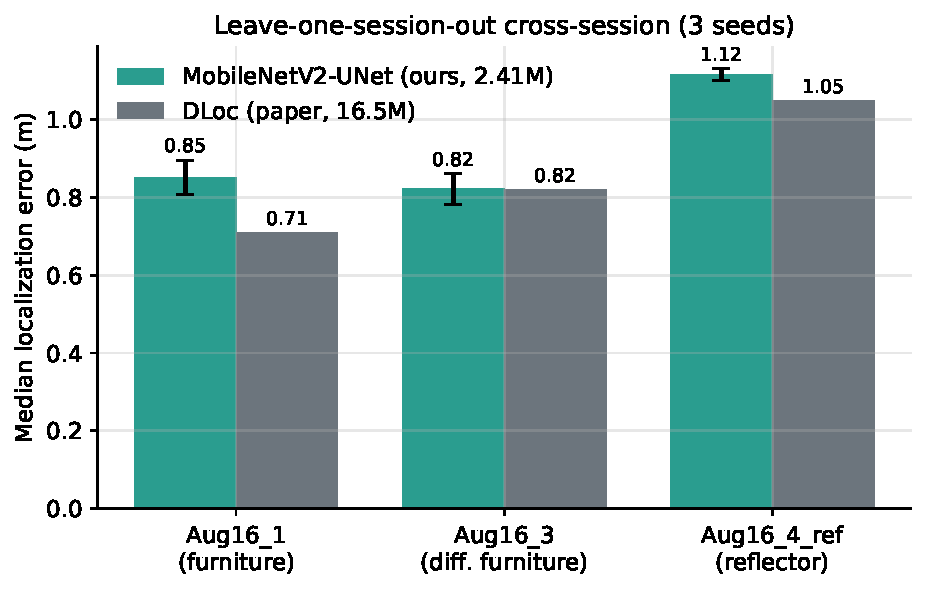
\includegraphics[width=0.62\textwidth]{crosssession_median.pdf}
\caption{Leave-one-session-out median error: our 2.41M-parameter MobileNetV2-UNet (three-seed mean $\pm$ std) against the published 16.5M-parameter DLoc. The U-Net matches DLoc on the different-furniture fold and lands within 0.14\,m on the others.}
\label{fig:crosssession_median}
\end{figure}

\subsection{Zero-shot stress test}
\label{sec:zeroshot}
The zero-shot protocol removes the held-out sessions from training entirely. Each model is trained only upon the two July sessions, then evaluated upon the three August sessions. This is purposely \emph{not} a fair comparison against DLoc; this is merely an internal ablation to reveal the contribution of each model component in the presence of an environmental shift. Table~\ref{tab:zeroshot} reports the results of each model variant on the unseen August sessions.

\begin{table}
\caption{Zero-shot cross-session accuracy (July-only training). Cells: median\,/\,P90 (m); best in \textbf{bold}.}
\label{tab:zeroshot}
\centering
\begin{tabular}{l l c c c}
\hline
\textbf{Model} & \textbf{Mode} & \textbf{Aug16\_1} & \textbf{Aug16\_3} & \textbf{Aug16\_4\_ref} \\
\hline
MobileNetV2      & Standalone & 1.118\,/\,3.138 & 1.204\,/\,3.471 & 1.500\,/\,3.367 \\
MobileNetV2      & Distilled  & 1.118\,/\,3.228 & 1.204\,/\,3.342 & 1.442\,/\,3.711 \\
MobileNetV2-UNet & Standalone & 1.063\,/\,2.508 & 1.005\,/\,3.704 & 1.334\,/\,3.301 \\
MobileNetV2-UNet & Distilled  & \textbf{1.020\,/\,2.319} & \textbf{1.005\,/\,2.608} & \textbf{1.281\,/\,3.002} \\
\hline
\end{tabular}
\end{table}

The results for the distilled MobileNetV2-UNet model reveal that it has the lowest median and P90 values for every session. The benefit of distillation is negligible on the furniture folds but becomes visible on the hardest (reflector) fold---both for the MobileNetV2 ($1.500 \to 1.442$\,m) and MobileNetV2-UNet ($1.334 \to 1.281$\,m) models. Thus, as discussed in section~\ref{sec:robustness}, the benefit of distillation becomes visible only when there is a shift of the data distribution. Finally, the TinyCNN model collapses entirely under this protocol (zero-shot medians of 5.964\,m, 6.327\,m, and 6.605\,m on the three August sessions), suggesting that under-capacity models do not merely lose accuracy in-distribution; they lose the ability to generalize at all.

\subsection{Furniture changes}
The two furniture folds are the mildest shift, and yet the compressed model handles them at deployable accuracy without any adaptation data. Under LOSO, the model localizes a rearranged furniture configuration (Aug16\_1) at a median error of 0.852\,m and a different furniture configuration (Aug16\_3) at 0.822\,m---indistinguishable from DLoc's 0.82\,m. Even for zero-shot furniture configurations, the model achieves median errors between 1.0 and 1.2\,m. Furniture rearrangement perturbs the multipath profile diffusely but leaves the dominant AoA/ToF geometry intact; both protocols find that the 2.41\,M-parameter model retains enough of that geometry to accurately localize the object.

\subsection{Reflector-induced multipath}
The aluminum reflector (Aug16\_4\_ref) is the hardest condition for every model in every protocol. The strong specular multipath introduced by the reflector's surface is seen in the scattered secondary peaks in figure~\ref{fig:heatmaps_cross} and in the reflector's CDF in figure~\ref{fig:cdf_cross}. Under LOSO, the U-Net's gap to DLoc is largest here (a median of 1.116\,m versus 1.05\,m for DLoc). The reason is architectural: the consistency (offset) decoder in DLoc helps to enforce consistency across the access points' estimates, which is beneficial under specular reflection, but the single-decoder student does not have such a decoder. Yet the student achieves a lower P90 of 2.489\,m compared to 2.77\,m for DLoc on this fold. Thus, while the skip connections help keep the tail of the distribution in check, the missing decoder has a small impact on the median performance of the student model.

\begin{figure}
\centering
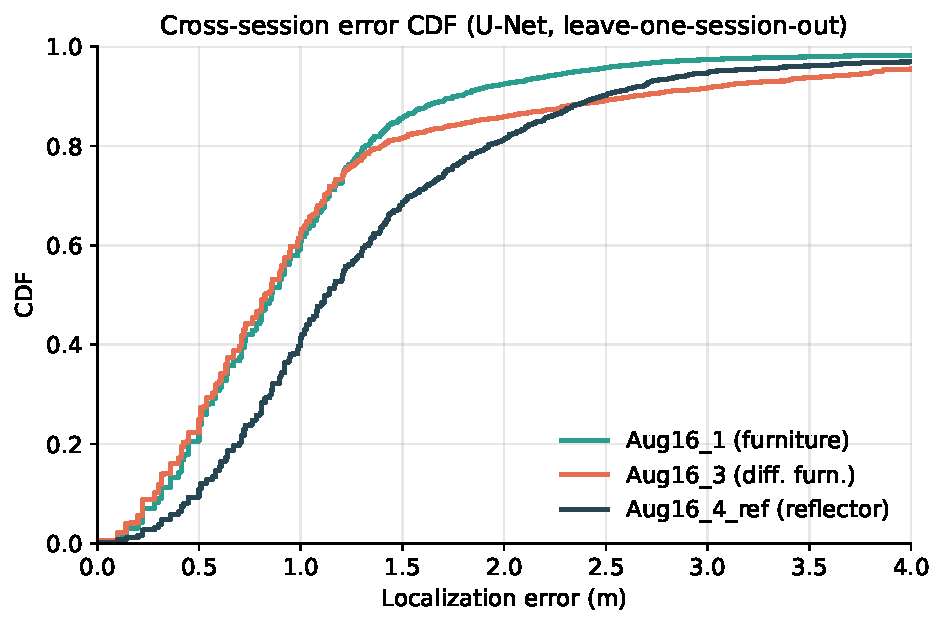
\includegraphics[width=0.62\textwidth]{cdf_crosssession.pdf}
\caption{Cross-session error CDFs for the three held-out folds. The reflector fold (Aug16\_4\_ref) is clearly the hardest, with its distribution shifted to larger errors, while the two furniture folds track closely.}
\label{fig:cdf_cross}
\end{figure}

\begin{figure}
\centering
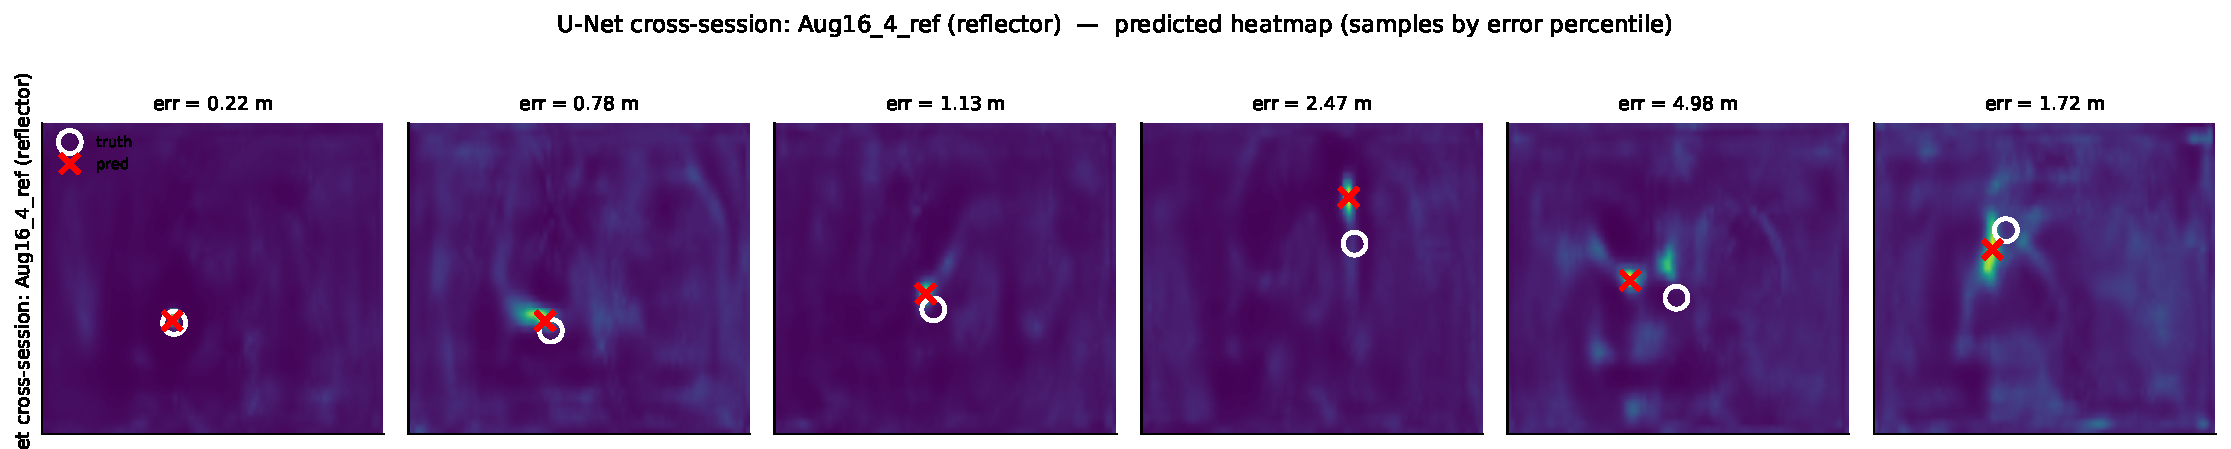
\includegraphics[width=\textwidth]{heatmaps_unet_cross_env4.pdf}
\caption{Qualitative cross-session predictions on the reflector fold (Aug16\_4\_ref). Compared with the in-distribution panels of figure~\ref{fig:heatmaps_indist}, the heatmaps show additional scattered probability mass---the specular ``phantom'' reflections introduced by the aluminum panel---which drives the larger errors on this fold.}
\label{fig:heatmaps_cross}
\end{figure}

\subsection{Environmental shifts and implications for deployment}
Across both protocols, the order of errors for every model is the same: in-distribution $<$ furniture folds $<$ reflector fold. Thus, the difficulty hierarchy is a property of the environment in which the models are deployed---not of the models themselves. Four consequences of this finding exist for model deployment. First, there is no trade-off between model compression and generalization. As the compressed U-Net and DLoc model degrade at the same rate in the face of environmental shift, the model that can fit on the edge device is the same that will survive shifts to the building environment. Second, adaptation data matters most where the physics of the environment changes: when a strongly reflective surface is introduced, either fine-tuning data from the changed environment (the LOSO setting, median of 1.116\,m) or an explicit cross-AP consistency mechanism is needed to close the gap relative to zero-shot operation (1.281\,m); therefore, integrating a consistency decoder into the student network is one possible next step. Third, based upon these findings, the model deployment should match the expected failure mode (section~\ref{sec:robustness}). Thus, the distilled MobileNetV2-UNet is the best model to deploy as a default model; it wins in every zero-shot test and is the most robust overall. The standalone model should only be deployed when very heavy noise on the received signal is the dominant concern. Finally, in terms of hardware requirements, the recommended model requires only 1.45\,GFLOPs and 27.2\,ms of CPU latency (section~\ref{sec:efficiency}); thus, the model can be deployed on AP or gateway hardware. Furthermore, since the model is relatively easy to retrain in each building, it can be recalibrated according to changes in that specific building's environment.

\section{Statistical stability and the accuracy--efficiency trade-off}
\label{sec:efficiency}
To confirm the gains in accuracy are not due to seed noise, the DLoc baseline was trained with three different seeds for the full 120 epochs (table~\ref{tab:multiseed}). The median error of $0.875 \pm 0.036$\,m for DLoc (coefficient of variation 4.1\%) is worse than the error after only 50 epochs due to the StepLR learning rate decay schedule ($\gamma{=}0.9$) that never decays the learning rate to zero over 120 epochs. Nevertheless, the MobileNetV2-UNet error of 0.640\,m is 6.5 standard deviations below the mean DLoc error for this setting. Furthermore, the P99 error of DLoc varies more between the three seeds (52\% coefficient of variation) since it depends upon locating a small number of inherently ambiguous locations on the map.

\begin{table}
\caption{Multi-seed DLoc baseline (120 epochs, StepLR $\gamma = 0.9$).}
\label{tab:multiseed}
\centering
\begin{tabular}{l c c c}
\hline
\textbf{Seed} & \textbf{Median (m)} & \textbf{P90 (m)} & \textbf{P99 (m)} \\
\hline
42  & 0.825 & 2.402 & 22.672 \\
123 & 0.906 & 2.335 &  7.714 \\
777 & 0.894 & 2.102 &  8.694 \\
\hline
Mean $\pm$ Std & $0.875 \pm 0.036$ & $2.280 \pm 0.128$ & $13.027 \pm 6.832$ \\
\hline
\end{tabular}
\end{table}

Regarding efficiency (table~\ref{tab:models} and figure~\ref{fig:params}), the MobileNetV2-UNet model uses fewer GFLOPs (1.45 compared to DLoc's 81.06, or $56\times$ less), takes less time to execute on CPU (27.2\,ms compared to DLoc's 270.9\,ms, or $10\times$ faster), and is $3.6\times$ faster on GPU. Thus, the accuracy--efficiency trade-off for this task is remarkably benign: accuracy does not decline with decreasing model size (the most accurate model in this paper is also $56\times$ cheaper than the baseline) until below 2\,M parameters, where the TinyCNN model offers a further $2.2\times$ reduction in the number of GFLOPs required for execution at the cost of a $6\times$ increase in median error. Thus, the gains in accuracy for MobileNetV2-UNet come at no computational cost, indicating that it is a strong candidate for deployment on edge devices.

\begin{figure}
\centering
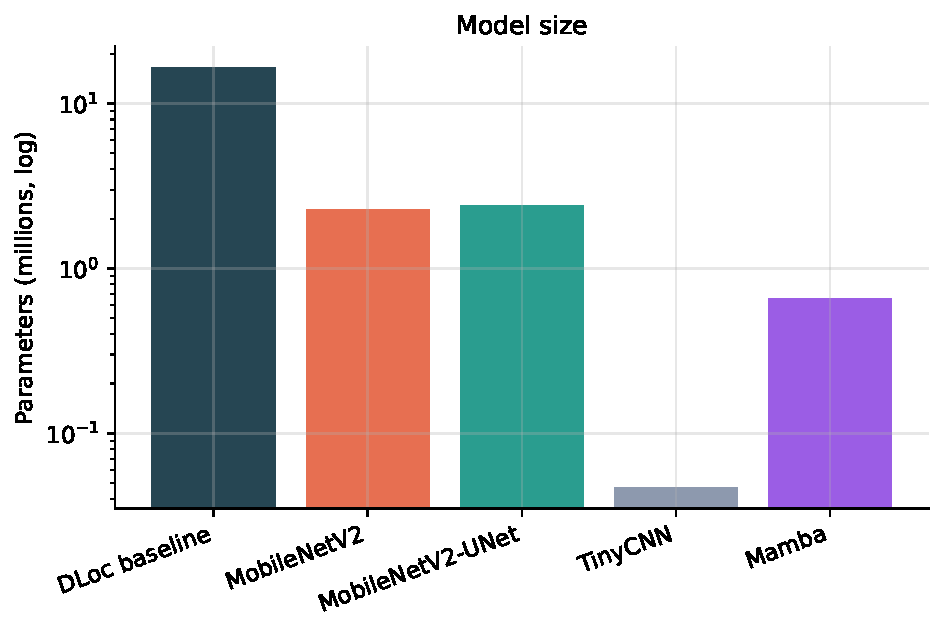
\includegraphics[width=0.6\textwidth]{compression_params.pdf}
\caption{Parameter counts of each model (log scale).}
\label{fig:params}
\end{figure}

\section{Conclusion}
\label{sec:conclusion}
We can now answer the six questions that we posed in section~\ref{sec:intro}.

\emph{How small can the model become before accuracy collapses?} Approximately 2 million parameters. MobileNetV2 has 2.27\,M parameters and matches our DLoc reproduction (0.707\,m median), while TinyCNN has 47\,K parameters but its median error is five times larger.

\emph{Does knowledge distillation recover lost accuracy?} No. Above the capacity floor, knowledge distillation is redundant within the distribution of training samples; below the floor, there is insufficient model capacity for knowledge distillation to compensate.

\emph{Which architectures preserve spatial localization?} Architectures that process the CSI as a 2D image. Mamba, for example, flattens the CSI signal into a 1D sequence and, therefore, cannot localize spatial features. U-Net models, however, use skip connections to preserve spatial information; a 2.41\,M parameter student model outperformed its 16.5\,M parameter teacher model (0.640\,m versus 0.707\,m for our reproduction, level with DLoc's published 0.64\,m).

\emph{Which models remain robust under signal degradation?} Models with U-Net skip connections are $5.5\times$ more robust to noise in the signal than models without them, and knowledge distillation provides $3.4\times$ robustness to noise as well as the best behavior under AP dropout for students above ${\sim}2$\,M parameters. These two mechanisms are complementary rather than additive, and below the capacity threshold distillation actively harms robustness.

\emph{Which models generalize across environmental changes?} The distilled MobileNetV2-UNet model exhibits the lowest median and P90 distances on every session that the model had never seen before. Furthermore, its standalone variant remained within 0.14\,m of DLoc on each session under DLoc's own leave-one-session-out protocol; the specular multipath caused by the reflector was the most difficult environmental change for all models to account for.

\emph{What is the accuracy--efficiency trade-off?} Benign down to the capacity floor: the recommended distilled MobileNetV2-UNet is simultaneously the most accurate and $56\times$ cheaper in FLOPs and $10\times$ faster on CPU than DLoc.

The overall conclusion is that DLoc-class accuracy does not require a DLoc-class model: the limit of model compression is instead constrained by a capacity floor of around 2\,M parameters and the requirement of a two-dimensional model architecture, not by the 16.5\,M parameters of the original system. Future work includes evaluating the recommended model on physical edge devices, collecting a CSI dataset of the E-JUST campus to evaluate performance across multiple buildings, conducting training with corrupted CSI samples to improve robustness to noise, incorporating a lightweight decoder to enforce consistency across APs into the student model, and extending the evaluation of the multi-seed approach to the student models.

\ack{The authors thank the authors of DLoc for releasing the WILD dataset publicly.}

\funding{This work received no external funding.}

\roles{Conceptualization and supervision: E.E. Methodology, software, investigation, validation, and writing (original draft): A.M.A.E., A.E.A.H.\ and F.Y.K.M. Writing (review and editing): all authors.}

\data{All code, trained weights, training logs, and pre-computed teacher outputs are openly archived. The source code is available at \href{https://github.com/JustAGek/DLoc-lightweight-localization}{github.com/JustAGek/DLoc-lightweight-localization}; the trained model weights and pre-processed dataset are mirrored on Hugging Face (links in the repository). The WILD dataset is publicly available from the DLoc authors~\cite{ayyalasomayajula2020deep}.}

\bibliographystyle{unsrt}
\bibliography{references}

\end{document}
